\documentclass[10pt]{beamer}

\usepackage[english]{babel}
\usepackage[utf8]{inputenc}
\usepackage[T1]{fontenc}
\usepackage{lmodern}

\usepackage{layout}
\usepackage{epsfig}
\usepackage{graphicx}
\graphicspath{{images/}}

\usepackage{siunitx}

\usepackage{amsthm}
\usepackage{amsmath}
\usepackage{amssymb}

\usepackage{mathrsfs}
\usepackage{wrapfig}
\usepackage{url}
\usepackage{multirow}
\usepackage{array}
\usepackage{pgfplots}

\usepackage[version=3]{mhchem}

\usepackage{wasysym}

%Bibtex
%\usepackage[square]{natbib}
%\newcommand{\newblock}{}

\usetheme{Warsaw}

\usepackage{graphicx}
\usepackage{epsfig}
\usepackage{epstopdf}
%\DeclareGraphicsRule{.eps}{pdf}{.pdf}{`epstopdf #1}
%\pdfcompresslevel=9
%\epstopdfsetup{suffix=}

\usepackage[]{algorithm2e}

\usepackage{todonotes}
\title{PageRank}
\author{
  Quentin Laurent
  \and
  Benoît Legat
}

\newcommand\bigoh{\mathcal{O}}

\usepackage{tikz}
\tikzstyle{vertex}=[circle,fill=gray!50,minimum size=15pt,inner sep=0pt]
\tikzstyle{visited}=[circle,fill=green!25,minimum size=15pt,inner sep=0pt]
\tikzstyle{unvisited}=[circle,fill=blue!25,minimum size=15pt,inner sep=0pt]



\begin{document}

\begin{frame}
  \maketitle
\end{frame}
\begin{frame}
  \tableofcontents
\end{frame}
\section{Introduction to pagerank}
\setbeamertemplate{background canvas}{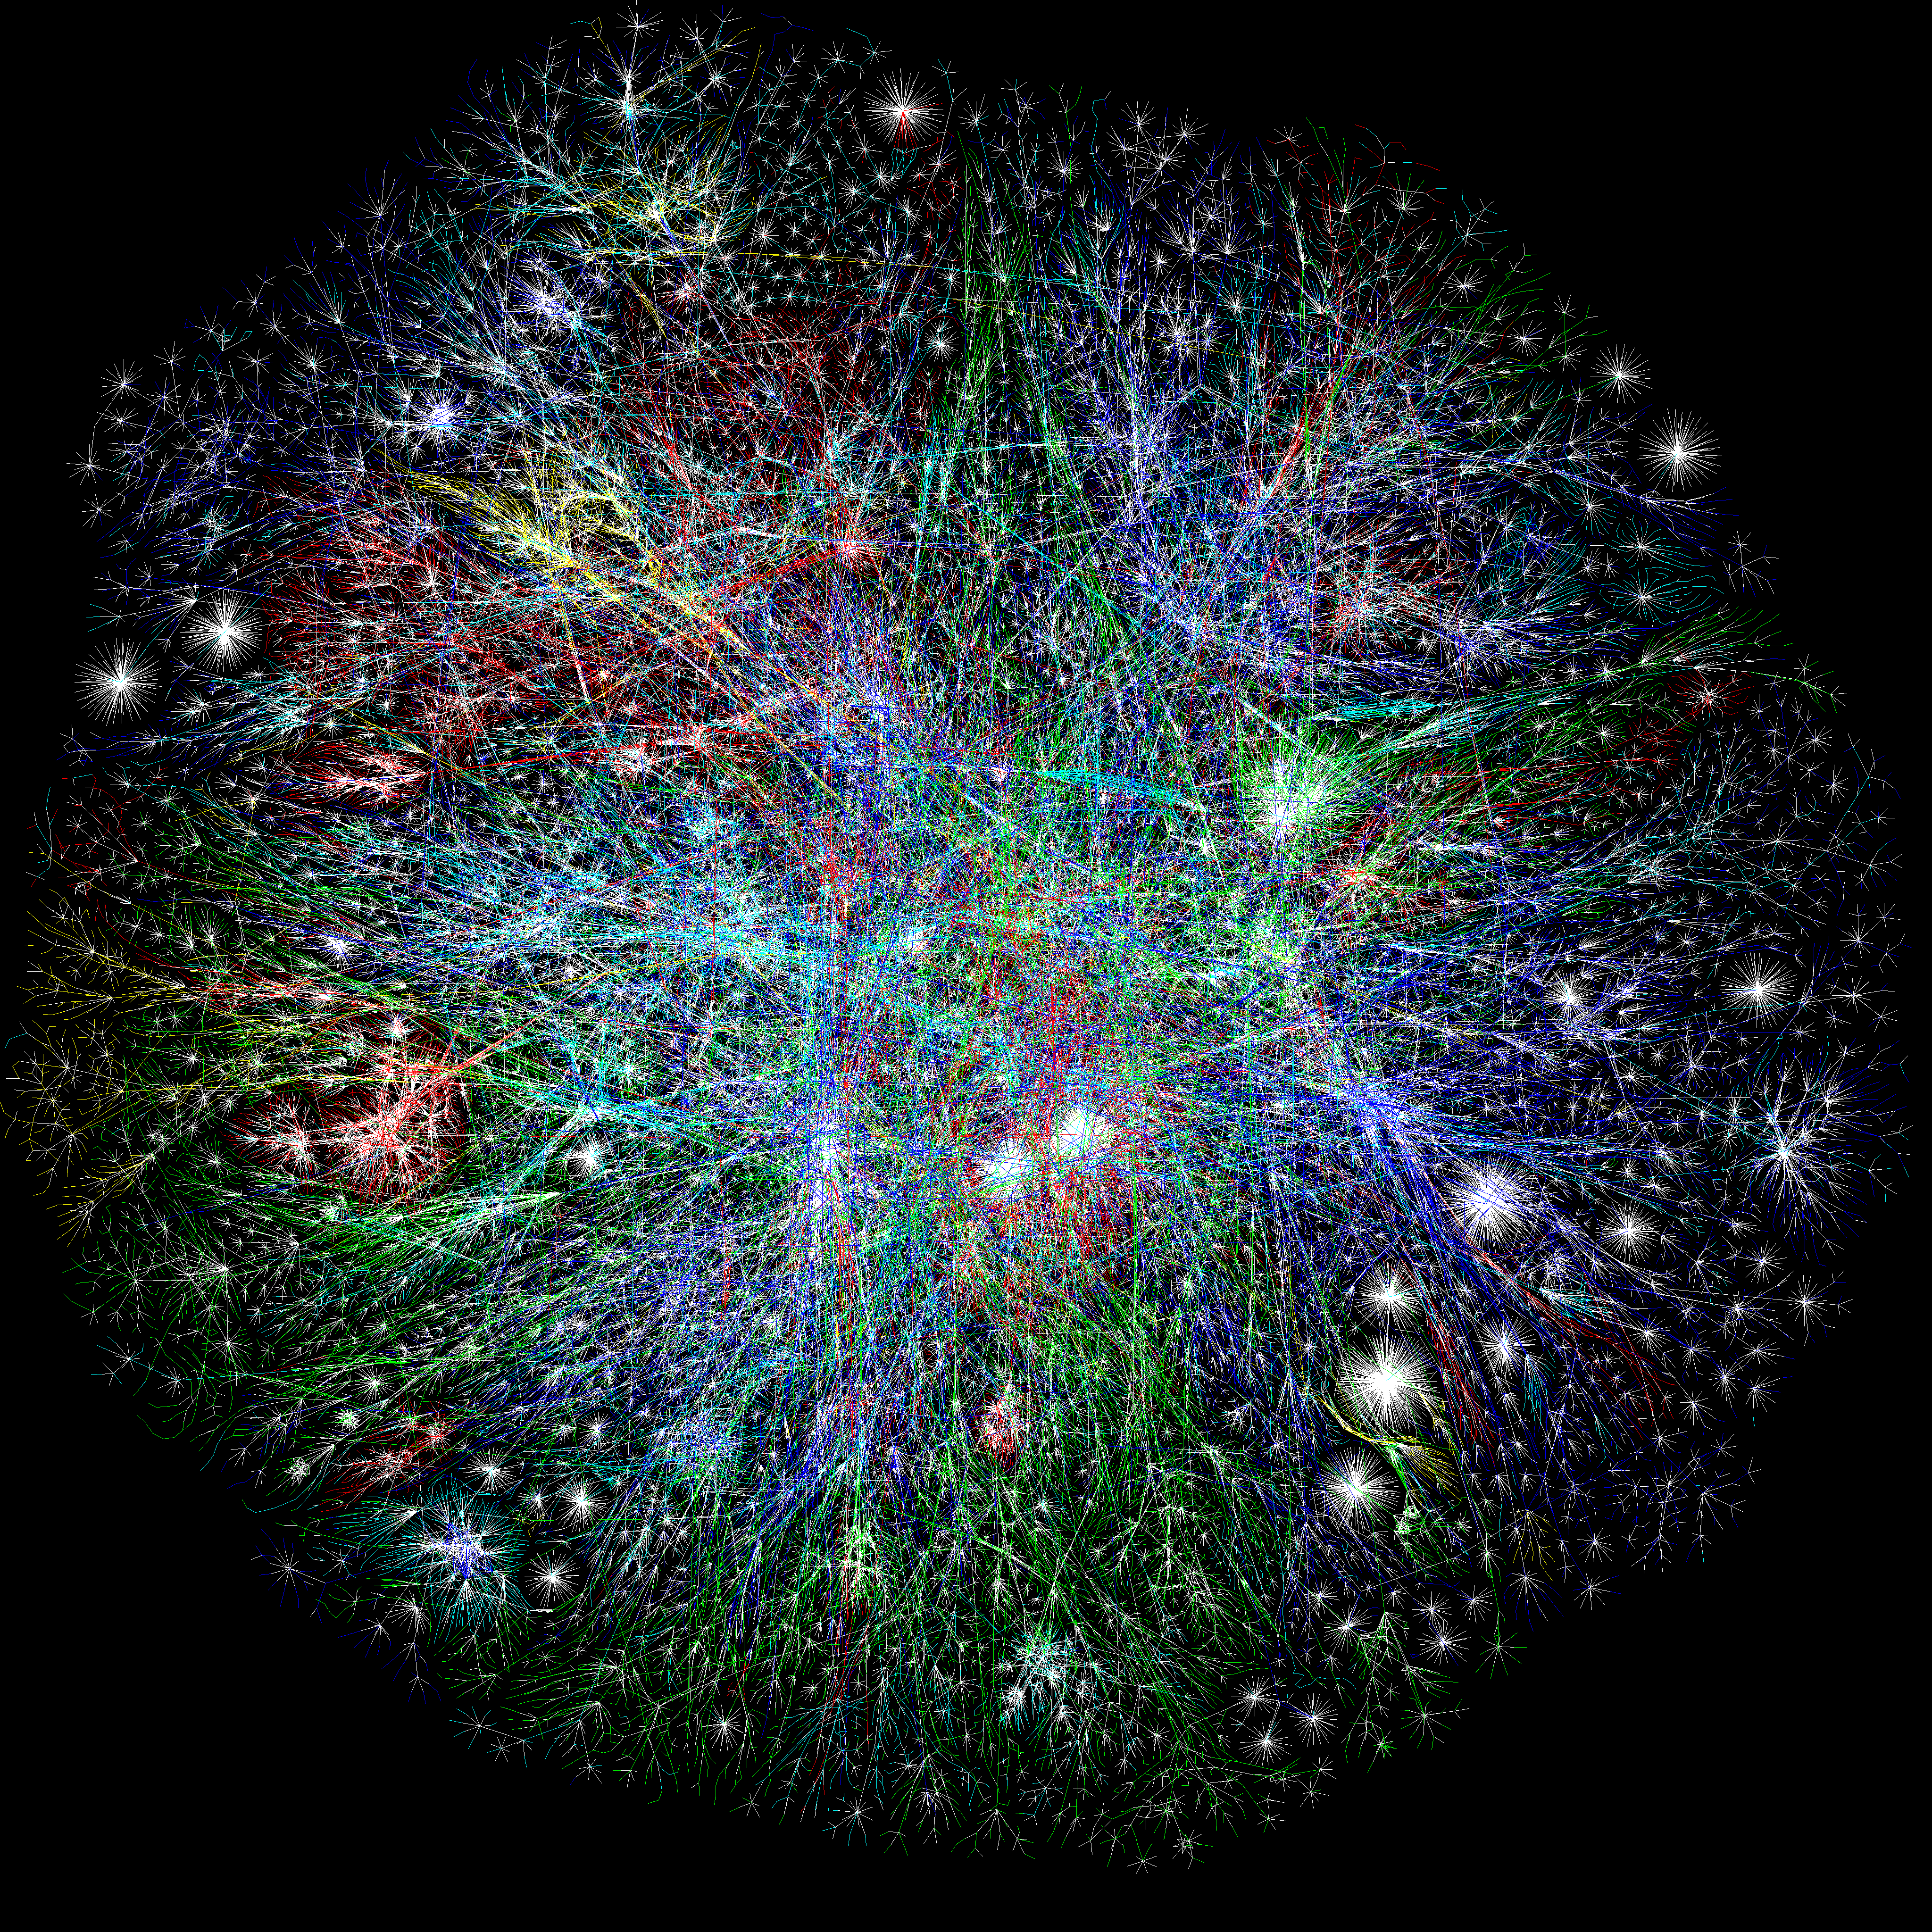
\includegraphics[width = \paperwidth]{InternetGraph.png}}
\setbeamertemplate{blocks}[rounded][shadow=false]
\begin{frame}
  \frametitle{Pagerank : motivation}
  \begin{block}{Where to start searching the web}
    How to find one's way through the millions of webpages of the web?
  \end{block}
  %\begin{figure}
  %	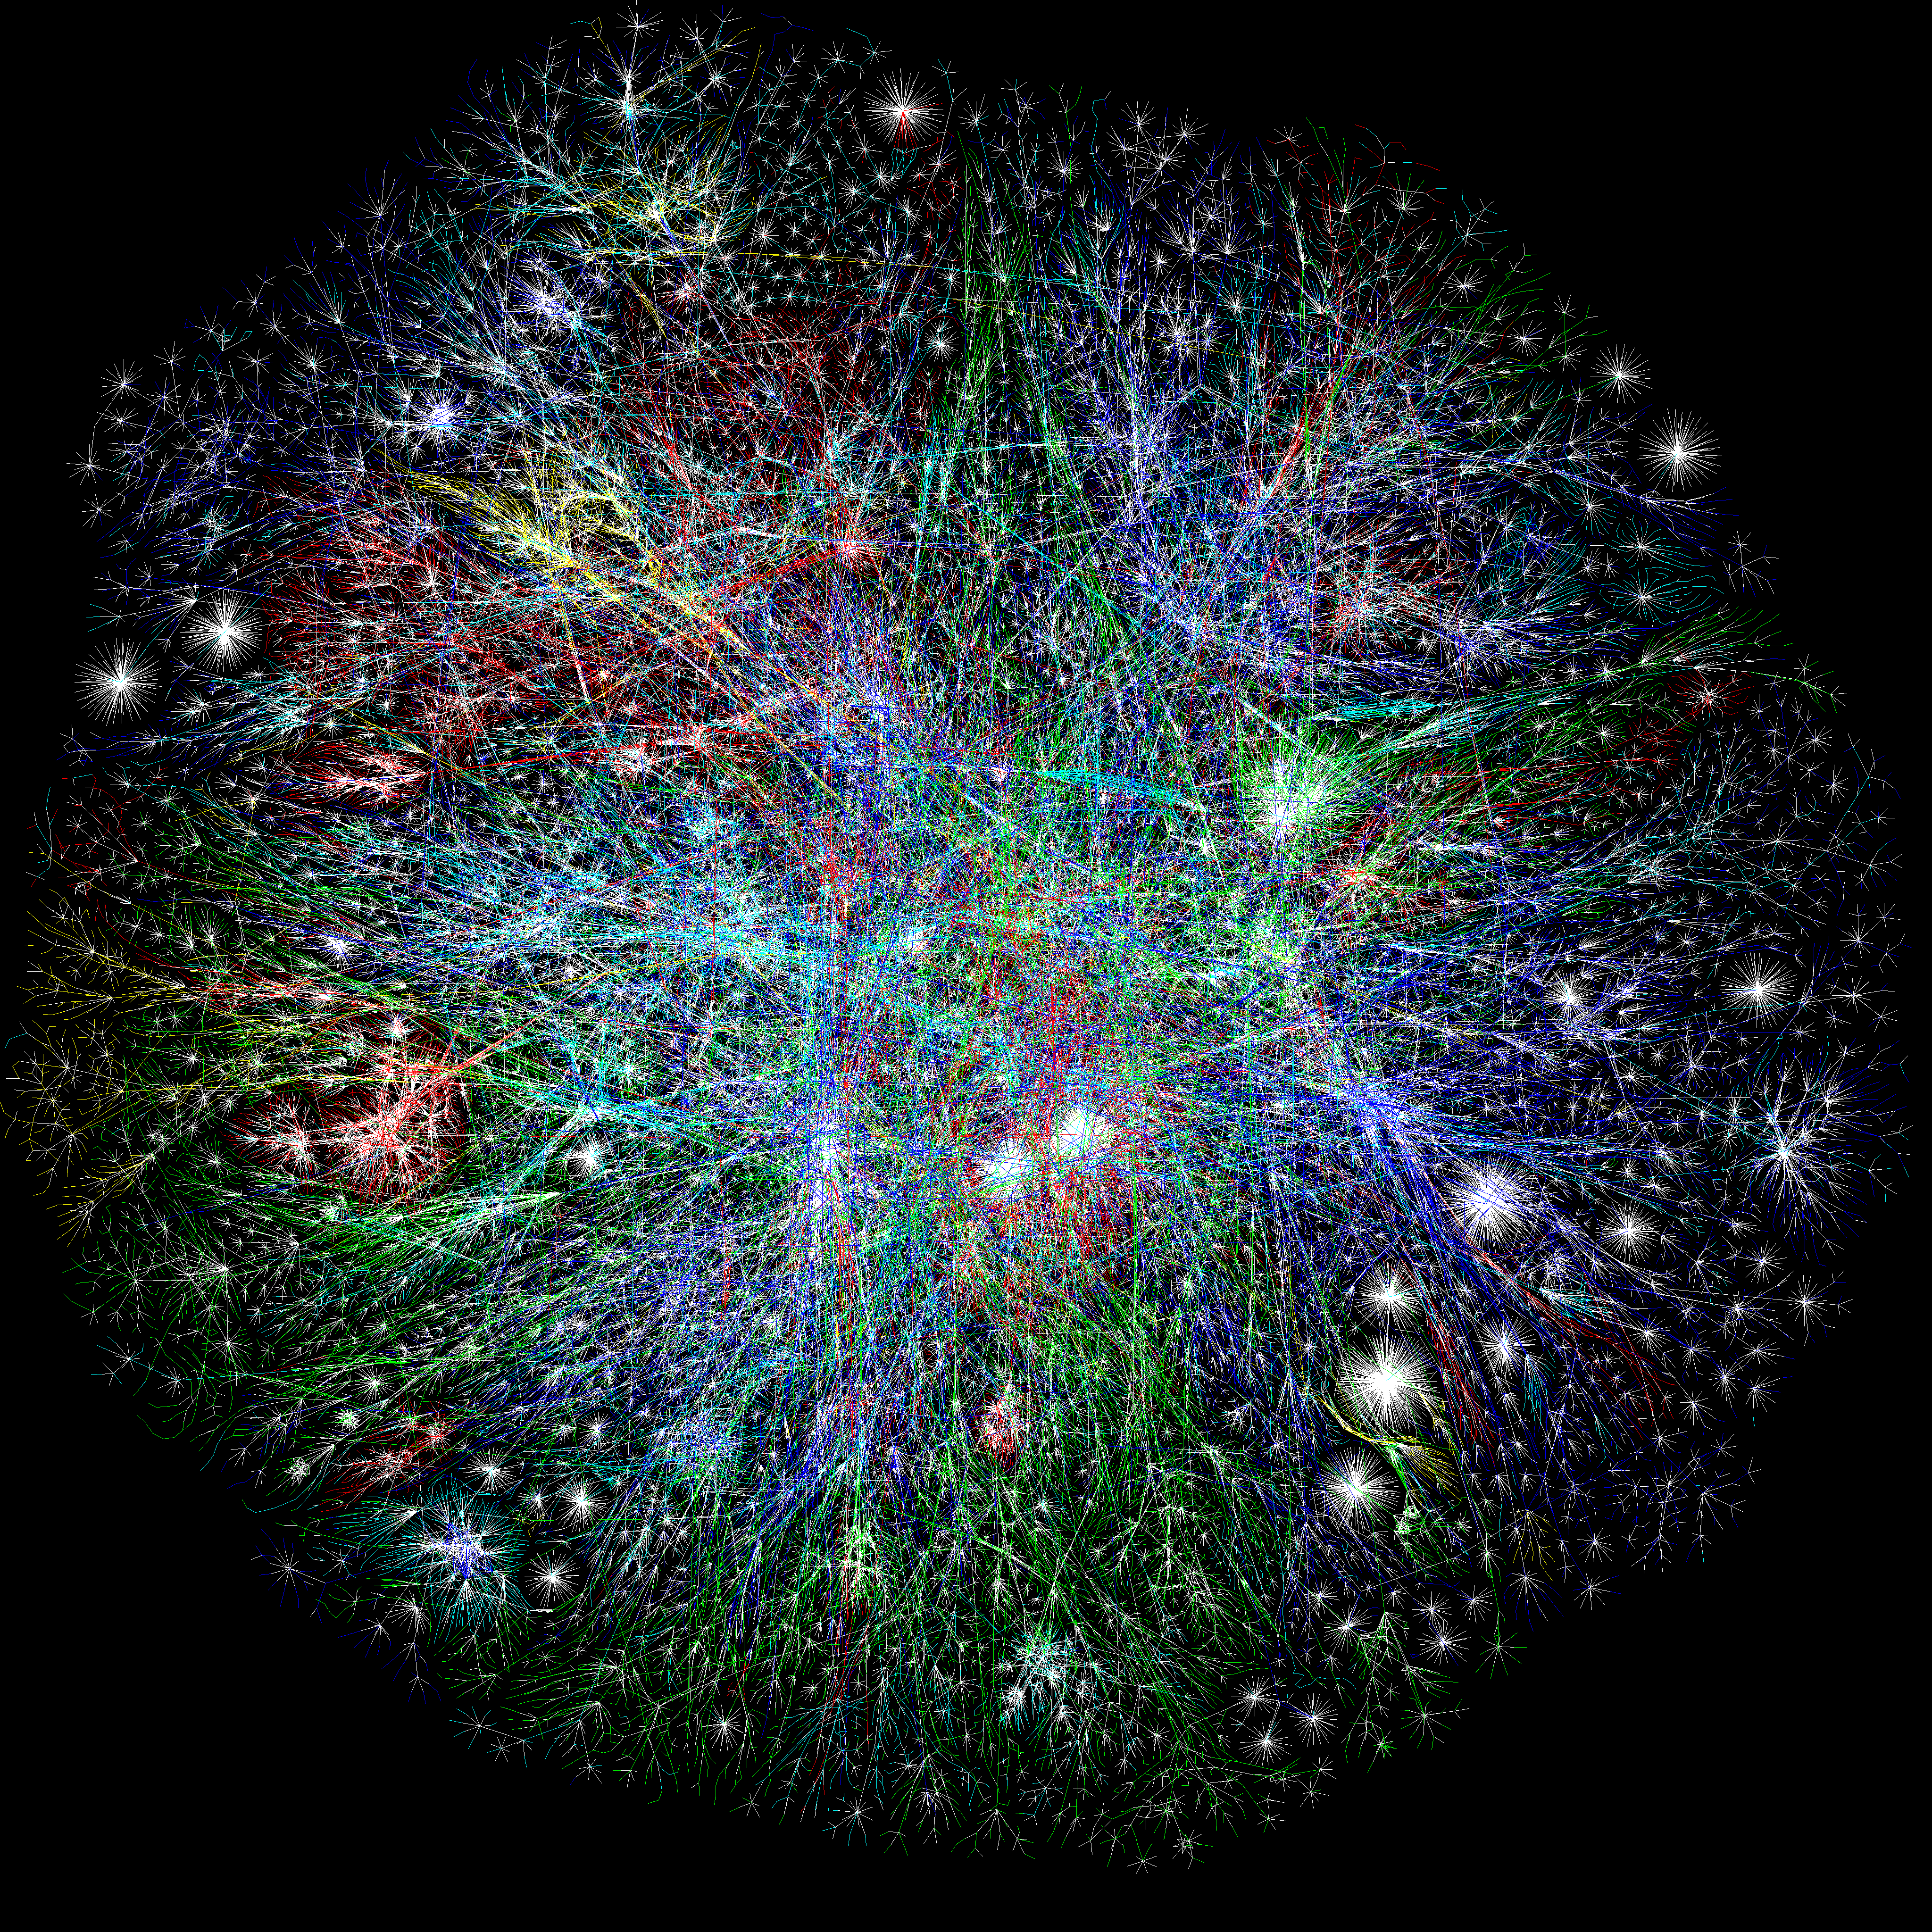
\includegraphics[width = 8cm]{InternetGraph.png}
  %	\end{figure}
  % Quentin
\end{frame}


\setbeamertemplate{background canvas}{}
\setbeamertemplate{blocks}[rounded][shadow=false]
\begin{frame}{Search engines}
  \begin{block}{Answer}
    \begin{itemize}
      \item Use of search engines
      \item Centralization : you only need to know the address of the search engine
    \end{itemize}
  \end{block}
  \begin{figure}
    \centering
    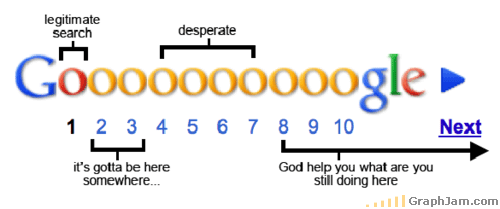
\includegraphics[width = 8cm]{google-search-result-pages.png}
  \end{figure}

\end{frame}


\begin{frame}{Early search engines}
  \begin{block}{At first}
    \begin{itemize}
      \item Early search engine's simply listed the terms in each page, making it easy to fool the search engine using \textbf{term spam}

    \end{itemize}
  \end{block}
  \begin{figure}
    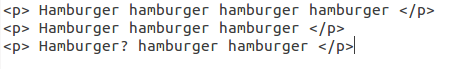
\includegraphics[width = 10cm]{termspam.png}
  \end{figure}
  \begin{block}{Pagerank}
    \begin{itemize}
      \item The game changed with Google's arrival and the use of this algorithm in search engines
    \end{itemize}
  \end{block}
\end{frame}


\setbeamertemplate{background canvas}{
\includegraphics[height = \paperheight]{surfer.png}}
\setbeamertemplate{blocks}[rounded][shadow=false]
\addtobeamertemplate{block begin}{\pgfsetfillopacity{0.7}}{\pgfsetfillopacity{1}}
\begin{frame}{The random web surfer}
  \begin{block}{PageRank takes in account}
    \begin{itemize}
      \item Likelihood of a random surfer to end up on a particular page 
      \item Content of a page related to the words used in the link to that page \textit{Todo : Comment on prend ça en compte?}
    \end{itemize}
    $\rightarrow$ The users of the web vote for the best pages by placing links to useful websites on their own sites\\
    $\rightarrow$ Has been proved to work empirically
  \end{block}
  %\begin{figure}
  %	
\includegraphics[width = 5cm]{surfer.png}
  %\end{figure}
\end{frame}

\setbeamertemplate{background canvas}{}
\setbeamertemplate{blocks}[shadow=true]
\section{Definition of pagerank}
\begin{frame}{Definition of pagerank}
  \begin{columns}
    \begin{column}{5cm}
      \begin{block}{The internet as a graph}
        Directed graph $\mathcal{G}$, pages are nodes and there is an arc from p1 to p2 if there is at least one link from p1 to p2
      \end{block}
    \end{column}
    \begin{column}{5cm}
      \begin{figure}[r]
        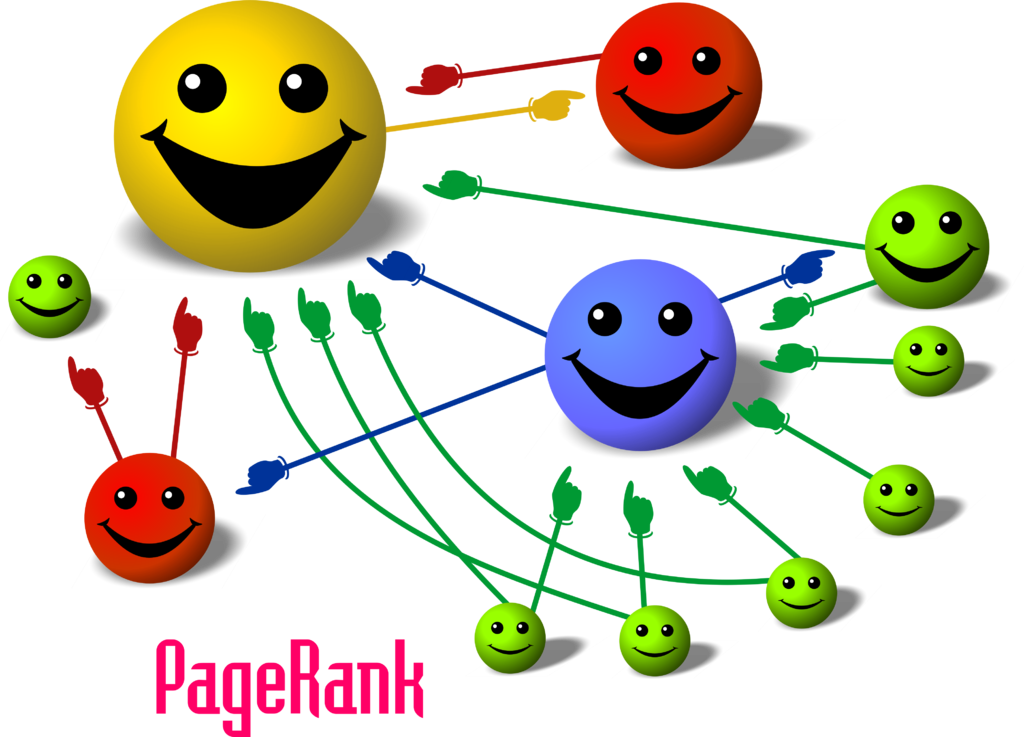
\includegraphics[width =4.5cm]{PageRank-hi-res.png}
      \end{figure}
    \end{column}
  \end{columns}
  \begin{definition}
    \begin{itemize}
      \item A function that assigns a real number to each page
      \item It corresponds to the probability of a random surfer of ending up on this particular page after an infinity of steps through the graph
    \end{itemize}
    $$Pgrk(\mathcal{G}) = v = \begin{vmatrix}v_0\\
      \vdots \\
    v_n\end{vmatrix} $$
  \end{definition}

\end{frame}


\begin{frame}{Construction of the transition matrix}
  \begin{block}{Transition matrix}
    \begin{itemize}
      \item Probability of one surfer of going to a linked page is $\frac{1}{l}$ where l is the amount of links leaving that page
      \item Henceforth the sum of the elements of each column is always 1 if there is at least one vertex leaving each page
    \end{itemize}
  \end{block}
  \begin{columns}
    \begin{column}{\paperwidth/2}
      \begin{figure}
        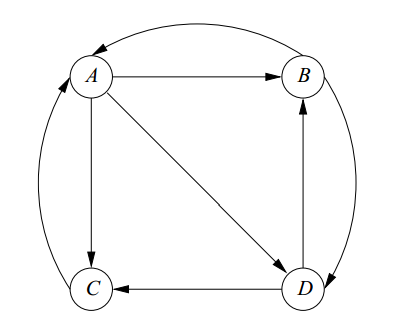
\includegraphics[width = 5cm]{graph1.png}
      \end{figure}
    \end{column}
    \begin{column}{\paperwidth/2}
      $$\begin{pmatrix}
        0 & \frac{1}{2} & 1 & 0 \\
        \frac{1}{3} & 0 & 0 &\frac{1}{2} \\
        \frac{1}{3} & \frac{1}{2}&  0& 0 

      \end{pmatrix}$$
    \end{column}
  \end{columns}
\end{frame}


\begin{frame}{Definition of pagerank}
  \begin{block}{Probability of distribution for the location of a random surfer}
    At first : $$v_0 = \begin{vmatrix}\frac{1}{n}\\
      \vdots \\
    \frac{1}{n}\end{vmatrix}$$
    Law of total probability : $P(A) = \sum_n P(A|B_n)P(B_n)$\\
    After 1 step, 2 steps, ... v becomes $Mv_0$, $M^2v_0$, ...
  \end{block}
  \begin{block}{Does it converge?}
    We approach a limiting distribution if the graph is strongly connected (hence there are no dead ends).\\
    v = Mv, v is the principal eigenvector \textit{Todo : proof}
    For the world wide web : 50-75 iterations are generally needed
  \end{block}
\end{frame}


\begin{frame}{Application to search engine}
  \begin{itemize}
    \item \textbf{Collect the data} Web crawlers
    \item \textbf{Selection of pages} A page needs to satisfy certain criteria to be considered in the pagerank, then other properties are used to determine (ex : search terms in prominent places)
    \item \textbf{Computation of pagerank} The algorithm described is used to associate a number to each page
    \item \textbf{Determination of the order on the result page} Each search engine has a secret formula in which pagerank plays an important role
  \end{itemize}
\end{frame}



\begin{frame}{Strongly Connected Components}
  \begin{columns}
    \begin{column}{0.4\textwidth}
      \begin{itemize}
        \item Strongly Connected Components (SCC) : $\exists$ path $u \to v$ $\forall u,v \in \mathsf{SCC}$.
        \item Component graph is a Directed Acyclic Graph (DAG).
        \item Computed on $\bigoh(|V| + |E|)$ with DFS (Tarjan or CLRS).
          They also toposort the DAG.
      \end{itemize}
    \end{column}
    \begin{column}{0.6\textwidth}
      \begin{center}
        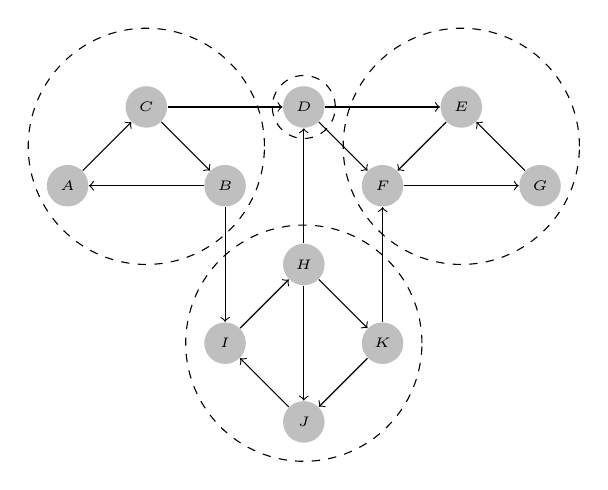
\begin{tikzpicture}
          \node[vertex] at (0, 0) (A) {\tiny $A$};
          \node[vertex] at (2, 0) (B) {\tiny $B$};
          \node[vertex] at (1, 1) (C) {\tiny $C$};
          \node[vertex] at (3, 1) (D) {\tiny $D$};
          \node[vertex] at (5, 1) (E) {\tiny $E$};
          \node[vertex] at (4, 0) (F) {\tiny $F$};
          \node[vertex] at (6, 0) (G) {\tiny $G$};
          \node[vertex] at (3, -1) (H) {\tiny $H$};
          \node[vertex] at (2, -2) (I) {\tiny $I$};
          \node[vertex] at (3, -3) (J) {\tiny $J$};
          \node[vertex] at (4, -2) (K) {\tiny $K$};

          \draw[->] (A) edge (C);
          \draw[->] (C) edge (B);
          \draw[->] (B) edge (A);
          \draw[->] (C) edge (D);
          \draw[->] (D) edge (E);
          \draw[->] (D) edge (F);
          \draw[->] (E) edge (F);
          \draw[->] (F) edge (G);
          \draw[->] (B) edge (I);
          \draw[->] (K) edge (F);
          \draw[->] (I) edge (H);
          \draw[->] (H) edge (K);
          \draw[->] (K) edge (J);
          \draw[->] (J) edge (I);
          \draw[->] (H) edge (J);
          \draw[->] (H) edge (D);
          \draw[->] (G) edge (E);

          \draw[dashed] (1, 0.5) circle (1.5);
          \draw[dashed] (5, 0.5) circle (1.5);
          \draw[dashed] (3, -2) circle (1.5);
          \draw[dashed] (3, 1) circle (0.4);
        \end{tikzpicture}
      \end{center}
    \end{column}
  \end{columns}
  \begin{center}
    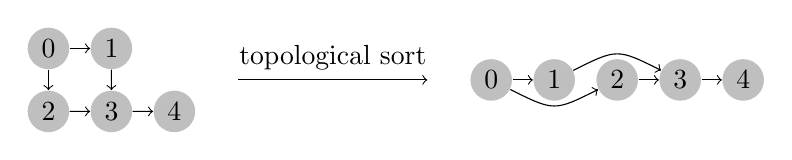
\begin{tikzpicture}[scale = 0.8]
      \begin{scope}[xshift=-100]
        \node[vertex] (n0) at (0, 0) {0};
        \node[vertex] (n1) at (1, 0) {1};
        \node[vertex] (n2) at (0, -1) {2};
        \node[vertex] (n3) at (1, -1) {3};
        \node[vertex] (n4) at (2, -1) {4};
        \draw[->] (n0) -- (n1);
        \draw[->] (n0) -- (n2);
        \draw[->] (n2) -- (n3);
        \draw[->] (n1) -- (n3);
        \draw[->] (n3) -- (n4);
      \end{scope}

      \begin{scope}
        \draw[->, anchor=south] (-0.5,-0.5) -- (1,-0.5) node{topological sort} -- (2.5,-0.5);
      \end{scope}

      \begin{scope}[xshift=100]
        \node[vertex] (n0) at (0, -0.5) {0};
        \node[vertex] (n1) at (1, -0.5) {1};
        \node[vertex] (n2) at (2, -0.5) {2};
        \node[vertex] (n3) at (3, -0.5) {3};
        \node[vertex] (n4) at (4, -0.5) {4};
        \draw[->] (n0) -- (n1);
        \draw[->] (n0) .. controls (1,-1) .. (n2);
        \draw[->] (n2) -- (n3);
        \draw[->] (n1) .. controls (2,0) .. (n3);
        \draw[->] (n3) -- (n4);
      \end{scope}
    \end{tikzpicture}
  \end{center}
\end{frame}

\begin{frame}{Actual Web graph}
  \begin{columns}
    \begin{column}{0.5\textwidth}
      \begin{itemize}
        \item One BIG SCC: ``Main SCC''.
        \item Tendrils out, Disconnected Components and Out Components:
          have at least one SCC with no arcs out.
          \begin{description}
            \item[dead end] only 1 page in the SCC.
            \item[spider strap] SCC with more than 1 page.
          \end{description}
        \item If Out Components is empty, Main SCC is a spider trap.
      \end{itemize}
    \end{column}
    \begin{column}{0.5\textwidth}
      \begin{figure}
        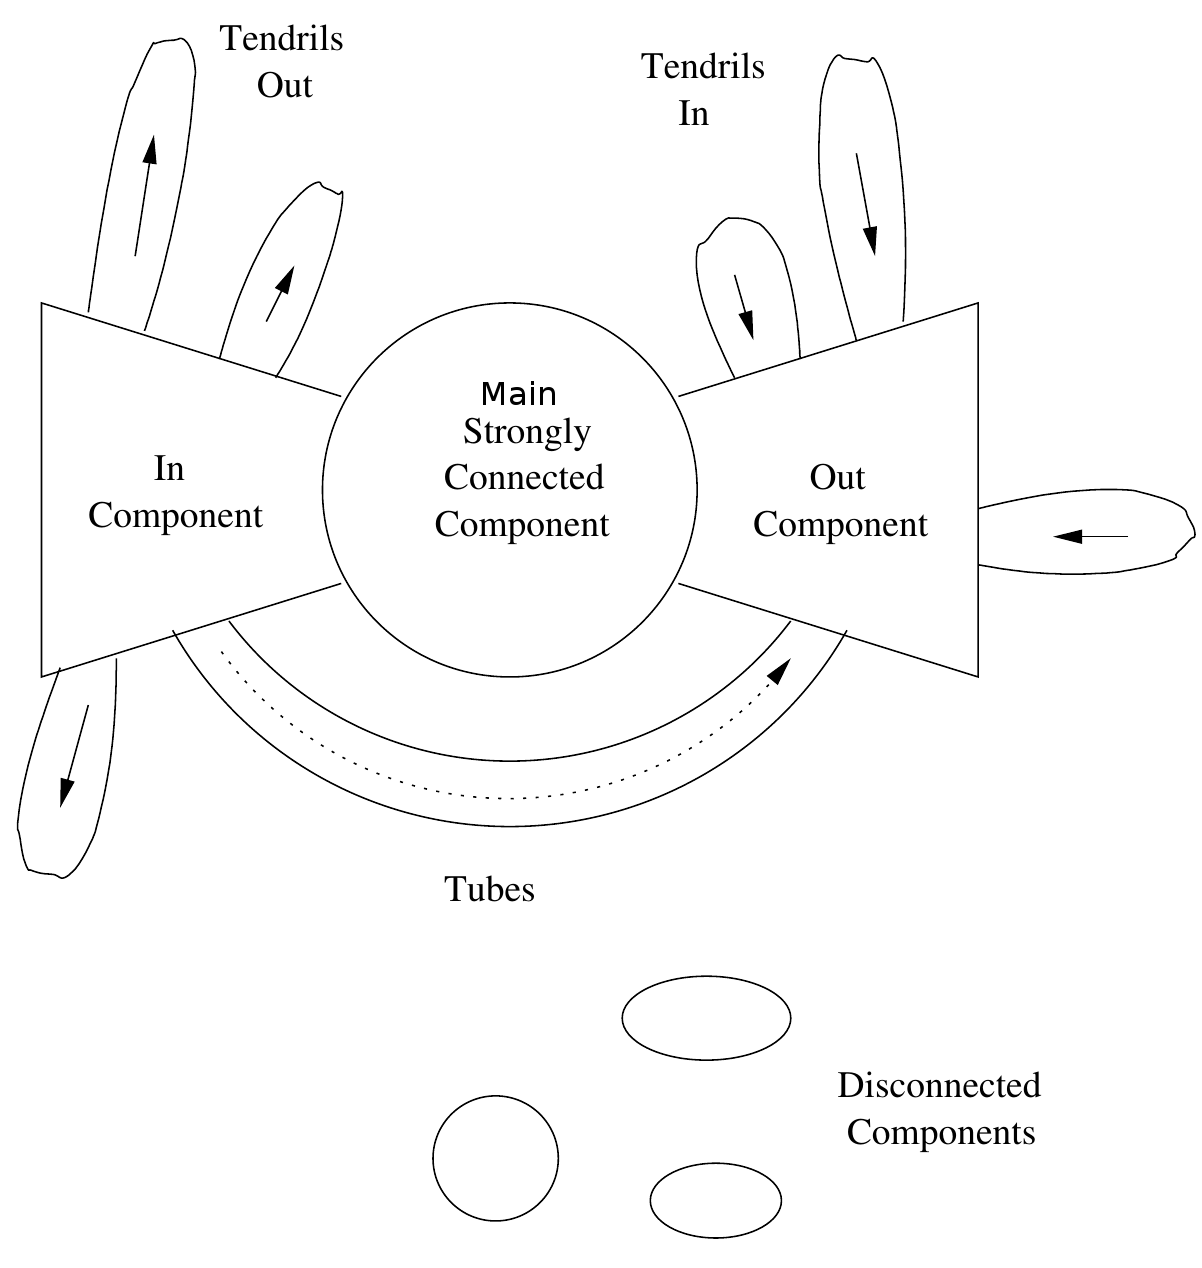
\includegraphics[trim=.5cm 0cm .2cm 0cm,clip,width=\linewidth]{web-graph.png}
        \caption{The ``bowtie'' picture of the Web \cite[p.~187]{leskovec2014mining} (modified).}
        \label{fig:web-graph}
      \end{figure}
    \end{column}
  \end{columns}
\end{frame}

\begin{frame}{Convergence of PageRank}
  \begin{block}{Sufficient condition}
    ``If the graph is \emph{strongly connected} and has no \emph{dead end}, $v$ converge to a limit such that $v = Mv$''
    \cite[p.~185]{leskovec2014mining}.
  \end{block}
  How can we have dead end in a SCC ?  Translation in our case:
  \begin{block}{Sufficient condition}
    ``In the Main SCC (everything else empty or removed), $v$ converge to a limit such that $v = Mv$''
    \cite[p.~185]{leskovec2014mining}.
  \end{block}
  % TODO PageRank defined only if there is a limit.. (proof that there is a limit if we start with 1,1,1.. :()
  %\begin{block}{Quid of dead ends ?}
  %PageRank of dead end is 0.
  %     We can have $v = Mv$. As we have seen, component of $v$ leading to a dead end will be 0.
  %     \begin{proof}
  %       By induction, if we have a dead end non-zero in $v$, since $v = Mv$, the sum of the components is unchanged so it is 0.
  %       Therefore, since $v = Mv$, the page linking to it are 0 too, ...
  %     \end{proof}
  %\end{block}
  %\begin{block}{Quid of spider trap ?}
  %  PageRank of spider trap is maybe not 0.
  %     \begin{proof}
  %       There exists a SCC without incoming link (since we have a DAG).
  %       \begin{itemize}
  %         \item If all of them are spider trap, we are done.
  %         \item Otherwise, 
  %       \end{itemize}
  %     \end{proof}
  %\end{block}
  % FIXME no need for convergence right now, I will prove it
  %       v_n = ...
  %       work with that
  Page rank of all pages is 0 except for pages in spider trap.
  \begin{proof}
    Take SCC with no in arcs, sum only gets smaller (no need for strict), therefore Cauchy.
    In $\mathbb{R}$ so in converges to $\epsilon$.
    $\epsilon \to 0$.
  \end{proof}
\end{frame}

\begin{frame}[allowframebreaks]{Solution 1 : pruning}
  \begin{algorithm}[H]
    \KwData{DAG $G$}
    \KwResult{Pruned $G$}
    \While{$G$ has a node $u$ with no arcs out}{
      remove incoming arcs of $u$\;
      remove $u$\;
    }
    \caption{Pruning a DAG}
  \end{algorithm}
  \begin{center}
    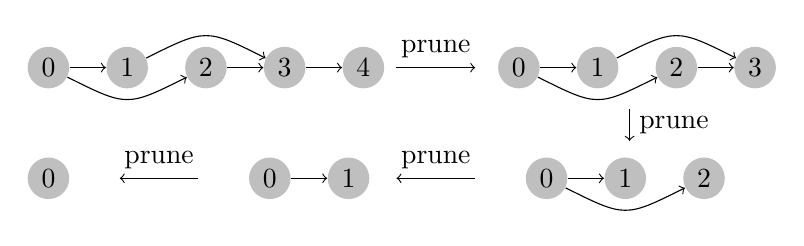
\begin{tikzpicture}
      \begin{scope}[xshift=-100]
        \node[vertex] (n0) at (0, -0.5) {0};
        \node[vertex] (n1) at (1, -0.5) {1};
        \node[vertex] (n2) at (2, -0.5) {2};
        \node[vertex] (n3) at (3, -0.5) {3};
        \node[vertex] (n4) at (4, -0.5) {4};
        \draw[->] (n0) -- (n1);
        \draw[->] (n0) .. controls (1,-1) .. (n2);
        \draw[->] (n2) -- (n3);
        \draw[->] (n1) .. controls (2,0) .. (n3);
        \draw[->] (n3) -- (n4);
      \end{scope}
      \begin{scope}[xshift=40]
        \draw[->, anchor=south] (-0.5,-0.5) -- (0,-0.5) node{prune} -- (0.5,-0.5);
      \end{scope}
      \begin{scope}[xshift=70]
        \node[vertex] (n0) at (0, -0.5) {0};
        \node[vertex] (n1) at (1, -0.5) {1};
        \node[vertex] (n2) at (2, -0.5) {2};
        \node[vertex] (n3) at (3, -0.5) {3};
        \draw[->] (n0) -- (n1);
        \draw[->] (n0) .. controls (1,-1) .. (n2);
        \draw[->] (n2) -- (n3);
        \draw[->] (n1) .. controls (2,0) .. (n3);
      \end{scope}
      \begin{scope}[xshift=110,yshift=-35]
        \draw[->, anchor=west] (0,0.2) -- (0,0) node{prune} -- (0,-0.2);
      \end{scope}
      \begin{scope}[xshift=80,yshift=-40]
        \node[vertex] (n0) at (0, -0.5) {0};
        \node[vertex] (n1) at (1, -0.5) {1};
        \node[vertex] (n2) at (2, -0.5) {2};
        \draw[->] (n0) -- (n1);
        \draw[->] (n0) .. controls (1,-1) .. (n2);
      \end{scope}
      \begin{scope}[xshift=40,yshift=-40]
        \draw[->, anchor=south] (0.5,-0.5) -- (0,-0.5) node{prune} -- (-0.5,-0.5);
      \end{scope}
      \begin{scope}[xshift=-20,yshift=-40]
        \node[vertex] (n0) at (0, -0.5) {0};
        \node[vertex] (n1) at (1, -0.5) {1};
        \draw[->] (n0) -- (n1);
      \end{scope}
      \begin{scope}[xshift=-60,yshift=-40]
        \draw[->, anchor=south] (0.5,-0.5) -- (0,-0.5) node{prune} -- (-0.5,-0.5);
      \end{scope}
      \begin{scope}[xshift=-100,yshift=-40]
        \node[vertex] (n0) at (0, -0.5) {0};
      \end{scope}
    \end{tikzpicture}
  \end{center}
  In our case, we need to stop at the Main SCC.
  $\bigoh(|V| + |E|)$ using the toposort order.

  \framebreak

  \begin{columns}
    \begin{column}{0.5\textwidth}
      \begin{block}{Interpretation}
        We only consider pages in the Main SCC or a page that \emph{indirectly} links to a page in the Main SCC.
      \end{block}
      Every node in the In Component will have PageRank 0.
    \end{column}
    \begin{column}{0.5\textwidth}
      \begin{figure}
        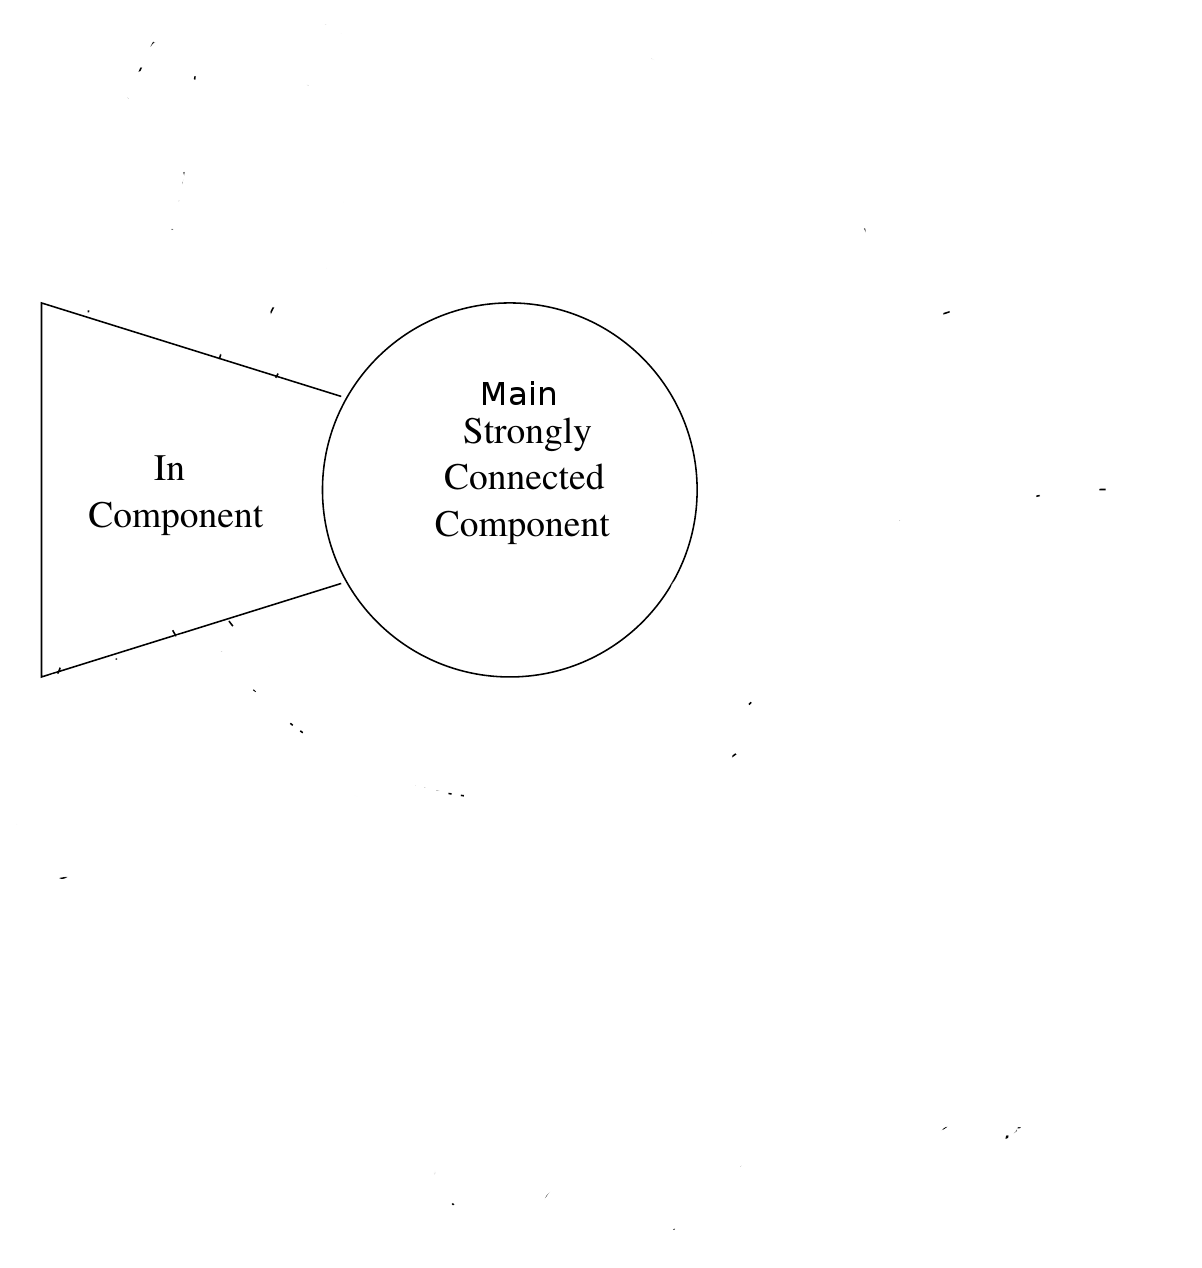
\includegraphics[trim=.5cm 0cm .2cm 0cm,clip,width=\linewidth]{web-graph-pruned.png}
        \caption{Pruned Web \cite[p.~187]{leskovec2014mining} (modified).}
        \label{fig:web-graph}
      \end{figure}
    \end{column}
  \end{columns}
\end{frame}

\begin{frame}{Solution 2 : Taxation}
\end{frame}

\begin{frame}{Topic sensitive}
  % Quentin
  \begin{block}{Biased random walks}
    \begin{itemize}
      \item Same principle as taxation
      \item This time we use a teleport set S relative to a certain topic
    \end{itemize}
    $$ v' = \beta Mv + (1-\beta)e_s/|S|$$
  \end{block}
\end{frame}


\begin{frame}{Deploying topic sensitive PageRank}
  \begin{block}{Steps for topic sensitive PageRank}
    \begin{itemize}
      \item Decide on the topics
      \item Pick a teleport set S
      \item Relate search queries with a topic(tricky : user chosen, webpages recently searched or bookmarks, facebook,...)
      \item Apply pagerank for selected topic(s)
    \end{itemize}
  \end{block}
\end{frame}

\begin{frame}{Hubs and Authorities}
\end{frame}


\section{Implementation}
\begin{frame}{Efficient representation of Transition Matrices}
  % Quentin
  \begin{block}{URLs and hyperlinks storage}
  \begin{itemize}
    \item Each URLs is associated with an integer
    \item M is sparse, represent it by its non-zero elements
    \item For each column : one integer for the out-degree, one integer per non-zero entry
  \end{itemize}
  \textbf{Todo : Application to topic sensitive}
\end{frame}

\begin{frame}{Use of MapReduce}
\begin{center}v  is too large to fit in main memory \end{center}
  \begin{block}{First approach}
    \begin{itemize}
      \item Separate v and separate M in k stripes
      \item Use of k map tasks whose sum is the result of a pagerank iteration
      \item The result v' will not fit in main memory either
    \end{itemize}
  \end{block}
  \begin{block}{Second approach : separate M in blocks}
    \begin{itemize}
      \item Separate v in k parts and M in $k^2$ squares.
      \item Use of $k^2$ map tasks, v is transmitted over the network k times
      \item Representing a column of blocks takes more space than a stripe but not too much (max 2 times more because of the repetition of the out degree)
    \end{itemize}
  \end{block}
\end{frame}

\begin{frame}
  \begin{thebibliography}{10}
      \beamertemplatebookbibitems
    \bibitem{leskovec2014mining}
      Leskovec, Jure and Rajaraman, Anand and Ullman, Jeffrey David
      A.~Autor.
      \newblock {\em Mining of massive datasets}.
      \newblock 2014.
      \newblock Cambridge University Press
      \beamertemplatearticlebibitems
  \end{thebibliography}
\end{frame}


\end{document}

% Sources images : 
% Gooooooogle : http://triooti.com/2014/08/23/google-nous-cache-des-informations-dans-les-recherches/
% Web graph : matthewgress.com
% Pagerank : wikipedia
